\subsection{Descrizione delle classi}

\subsubsection{Introduzione}
\par Il team ha creato un file di configurazione che utilizza il pattern \glossario{Singleton} per gestire le impostazioni dell'applicazione. La classe \textit{Configuration} è responsabile del caricamento e della gestione delle configurazioni, che vengono lette da un file \glossario{JSON} esterno. All'interno di questo file, è possibile definire le dipendenze esterne, tra cui \glossario{txtai} e \glossario{SQLAlchemy}, che saranno gestite dagli adapter. Inoltre, è previsto il supporto per parametri aggiuntivi, come i percorsi dei modelli di ricerca semantica per txtai. La classe Configuration offre un punto centrale di accesso alle configurazioni e ai servizi dell'applicazione, semplificando la gestione e l'organizzazione del codice.
\par La sezione seguente descrive le classi che compongono il \glossario{back-end} dell'applicazione. L'elenco segue la composizione dell'architettura, fornendo una descrizione degli attributi e dei metodi che caratterizzano ciascuna classe, insieme alle interfacce implementate e alle dipendenze verso altre classi del sistema.
\par La sezione principale è suddivisa in due sottosezioni:
\begin{itemize}
  \item \textbf{Incoming}: classi che preparano i dati per il core dell'applicazione;
  \item \textbf{Outcoming}: classi che interagiscono con servizi esterni. 
\end{itemize}

\vspace{0.5\baselineskip}
\par Le sezioni incoming e outcoming sono ulteriormente suddivise per distinguere tra porte, adapter e servizi. Le porte contengono le interfacce che vengono poi implementate dagli adapter o dai servizi.
\subsubsection{Ports - Incoming}

\subsubsubsection{AuthenticationUseCase} \label{AuthenticationUseCase}
\begin{figure}[H]
    \centering
    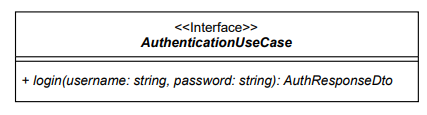
\includegraphics[width=0.6\textwidth]{assets/Backend/authentication_use_case.png}
    \caption{Diagramma dell'interfaccia AuthenticationUseCase}
  \end{figure}
\begin{itemize}
    \item \textbf{Descrizione}: AuthenticationUseCase definisce il contratto per i casi d'uso relativi all'autenticazione degli utenti;
    \item \textbf{Operazioni}:
    \begin{itemize}
        \item Autenticazione con username e password.
    \end{itemize}
    \item \textbf{Implementazione}: i dettagli dell'implementazione sono riportati nelle classi concrete.
\end{itemize}  

\subsubsubsection{DictionaryUseCase} \label{DictionaryUseCase}
\begin{figure}[H]
    \centering
    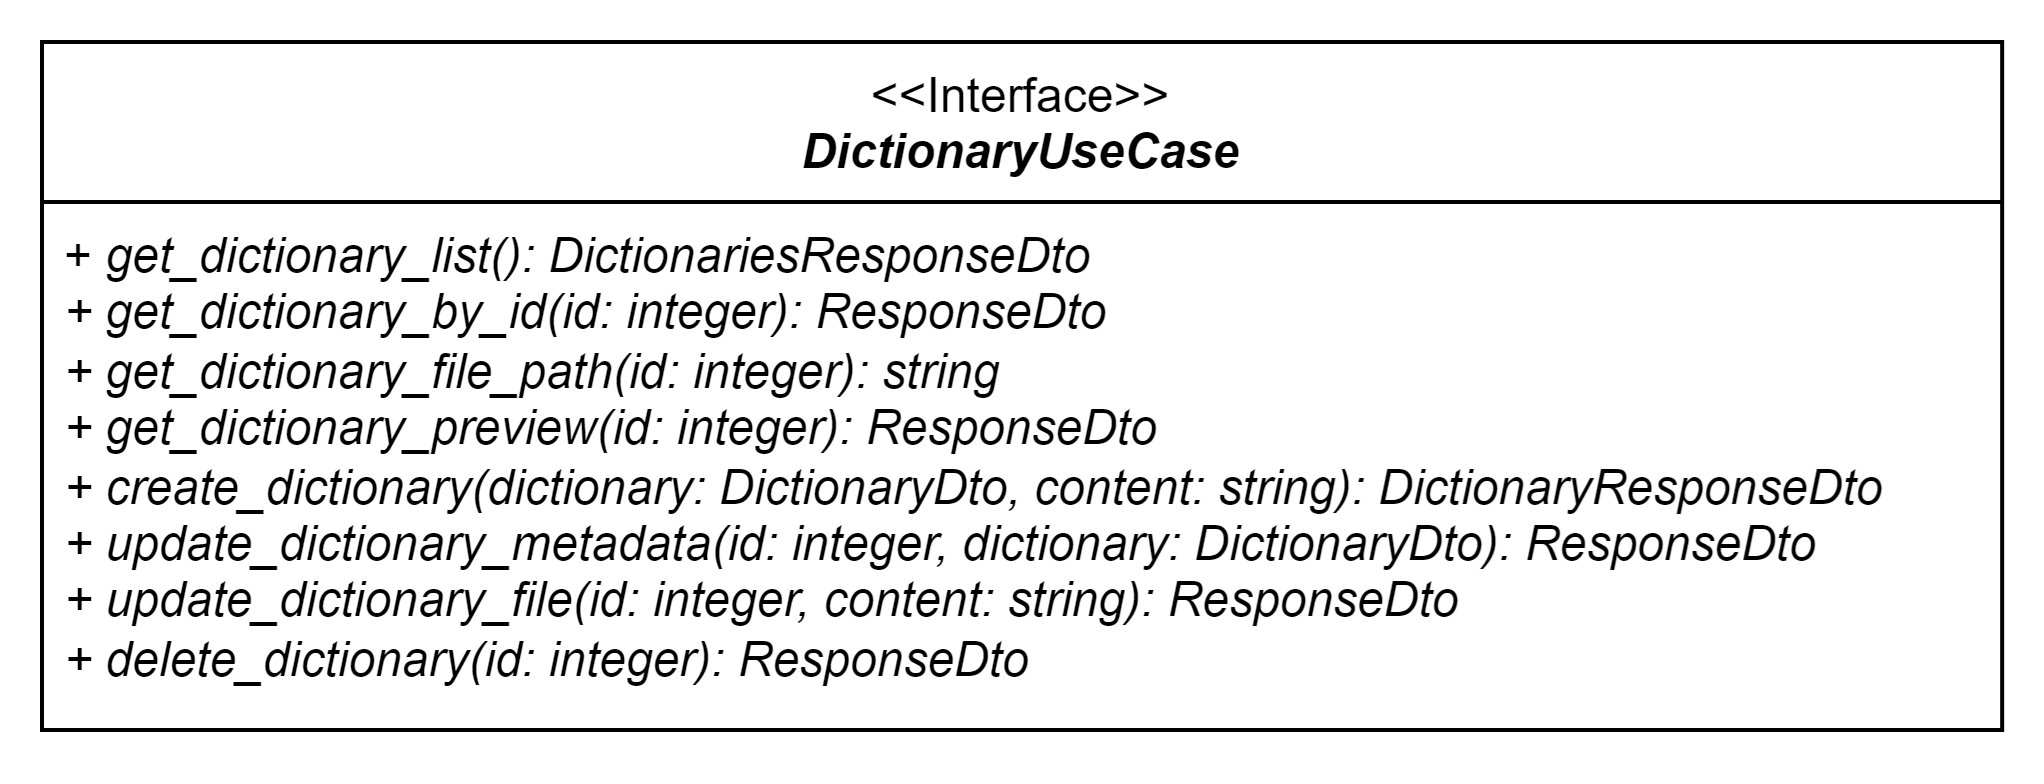
\includegraphics[width=0.7\textwidth]{assets/Backend/dictionary_use_case.png}
    \caption{Diagramma dell'interfaccia DictionaryUseCase}
  \end{figure}
\begin{itemize}
    \item \textbf{Descrizione}: DictionaryUseCase definisce il contratto per i casi d'uso relativi alle operazioni sui \glossario{dizionari dati};
    \item \textbf{Operazioni}:
    \begin{itemize}
      \item Recupero delle informazioni di tutti i dizionari;
      \item Recupero delle informazioni di un dizionario;
      \item Recupero del file di un dizionario;
      \item Anteprima di un dizionario;
      \item Creazione di un dizionario;
      \item Aggiornamento dei metadati di un dizionario;
      \item Aggiornamento del file di un dizionario;
      \item Eliminazione di un dizionario.
    \end{itemize}
    \item \textbf{Implementazione}: i dettagli dell'implementazione sono riportati nelle classi concrete.
\end{itemize}  

\subsubsubsection{PromptUseCase} \label{PromptUseCase}
\begin{figure}[H]
    \centering
    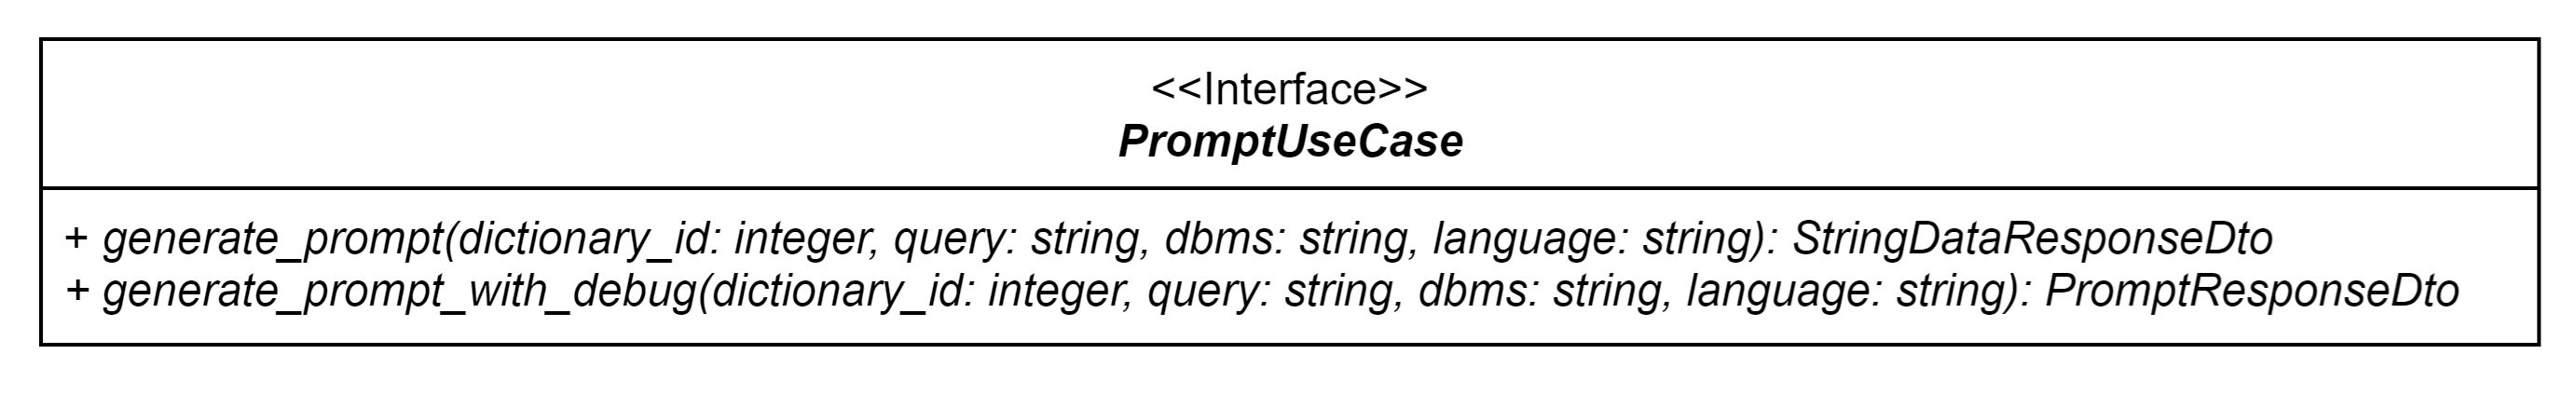
\includegraphics[width=0.8\textwidth]{assets/Backend/prompt_use_case.png}
    \caption{Diagramma dell'interfaccia PromptUseCase}
  \end{figure}
\begin{itemize}
    \item \textbf{Descrizione}: PromptUseCase definisce il contratto per i casi d'uso relativi alla generazione del \glossario{prompt};
    \item \textbf{Operazioni}:
    \begin{itemize}
      \item Generazione del prompt a partire da una richiesta, un dizionario, una lingua e un \glossario{DBMS};
      \item Generazione del prompt con informazioni di debug associate ad esso.
    \end{itemize}
    \item \textbf{Implementazione}: i dettagli dell'implementazione sono riportati nelle classi concrete.
\end{itemize}  

\subsubsubsection{SchemaValidatorUseCase} \label{SchemaValidatorUseCase}
\begin{figure}[H]
    \centering
    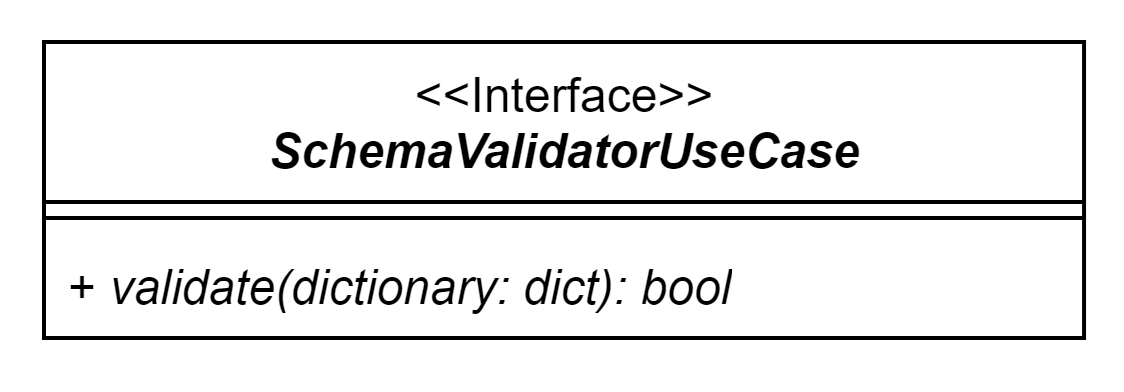
\includegraphics[width=0.6\textwidth]{assets/Backend/schema_validator_use_case.png}
    \caption{Diagramma dell'interfaccia SchemaValidatorUseCase}
  \end{figure}
\begin{itemize}
    \item \textbf{Descrizione}: SchemaValidatorUseCase definisce il contratto per i casi d'uso relativi alla validazione dello schema dei \glossario{dizionari dati};
    \item \textbf{Operazioni}:
    \begin{itemize}
      \item Validazione dello schema di un dizionario dati.
    \end{itemize}
    \item \textbf{Implementazione}: i dettagli dell'implementazione sono riportati nelle classi concrete.
\end{itemize}  

\subsubsubsection{Ports - Outcoming}

\subsubsubsection{EmbeddingsAbstractFactory} \label{EmbeddingsAbstractFactory}
\begin{figure}[H]
    \centering
    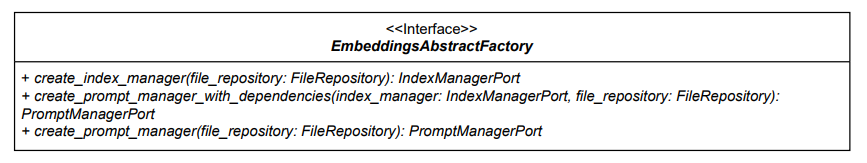
\includegraphics[width=0.5\textwidth]{assets/Backend/embeddings_abstract_factory.png}
    \caption{Diagramma dell'interfaccia EmbeddingsAbstractFactory}
  \end{figure}
\begin{itemize}
    \item \textbf{Descrizione}: EmbeddingsAbstractFactory fornisce una struttura per la creazione dei componenti relativi agli \glossario{embeddings} e alla generazione dei \glossario{prompt};
    \item \textbf{Operazioni}:
    \begin{itemize}
      \item Creazione di un'istanza di IndexManagerPort;
      \item Creazione di un'istanza di PromptManagerPort con le sue dipendenze;
      \item Creazione di un'istanza di PromptManagerPort delegando prima la creazione delle sue dipendenze.
    \end{itemize}
    \item \textbf{Implementazione}: i dettagli dell'implementazione sono riportati nelle classi concrete;
    \item \textbf{Dipendenze}:
    \begin{itemize}
        \item FileRepository;
        \item IndexManagerPort;
        \item PromptManagerPort.
    \end{itemize}
\end{itemize}  

\subsubsubsection{IndexManagerPort} \label{IndexManagerPort}
\begin{figure}[H]
    \centering
    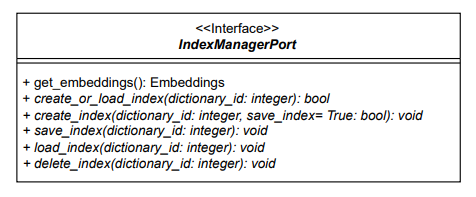
\includegraphics[width=0.6\textwidth]{assets/Backend/index_manager_port.png}
    \caption{Diagramma dell'interfaccia IndexManagerPort}
  \end{figure}
\begin{itemize}
    \item \textbf{Descrizione}: IndexManagerPort fornisce un'interfaccia per gestire le operazioni CRUD relative agli \glossario{embeddings};
    \item \textbf{Operazioni}:
    \begin{itemize}
      \item Recupero degli embeddings;
      \item Creazione di un indice;
      \item Salvataggio di un indice;
      \item Ripristino di un indice;
      \item Eliminazione di un indice.
    \end{itemize}
    \item \textbf{Implementazione}: i dettagli dell'implementazione sono riportati nelle classi concrete.
\end{itemize} 

\subsubsubsection{PromptManagerPort} \label{PromptManagerPort}
\begin{figure}[H]
    \centering
    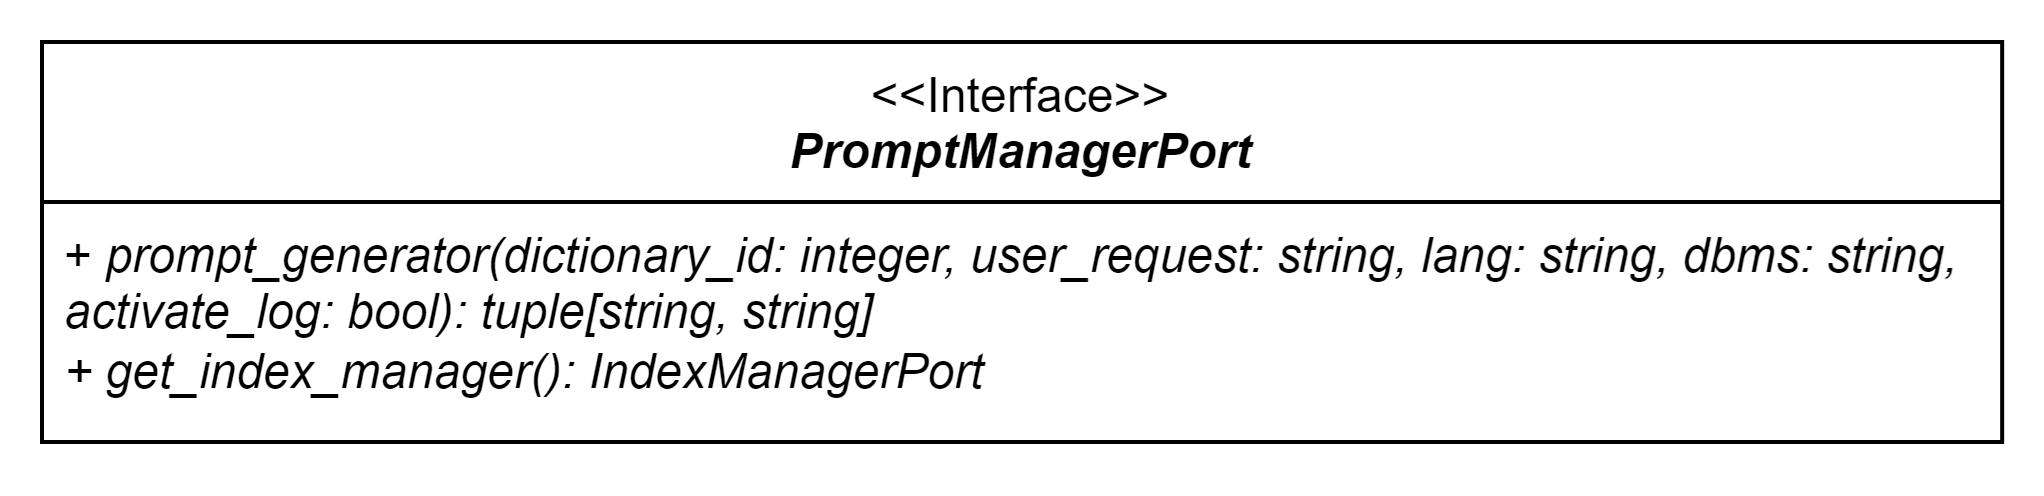
\includegraphics[width=0.6\textwidth]{assets/Backend/prompt_manager_port.png}
    \caption{Diagramma dell'interfaccia PromptManagerPort}
  \end{figure}
\begin{itemize}
    \item \textbf{Descrizione}: questa interfaccia si occupa del recupero delle informazioni e la generazione del prompt.
    \item \textbf{Operazioni}:
    \begin{itemize}
      \item Generazione del prompt;
      \item Recupero dell'istanza di IndexManagerPort;
      \item Creazione dell'istanza di DebugManagerPort.
    \end{itemize}
    \item \textbf{Implementazione}: i dettagli dell'implementazione sono riportati nelle classi concrete;
    \item \textbf{Dipendenze}:
    \begin{itemize}
        \item \texttt{IndexManagerPort};
        \item \texttt{DebugManagerPort}.
    \end{itemize}
\end{itemize} 

\subsubsubsection{DebugManagerPort} \label{DebugManagerPort}
\begin{figure}[H]
    \centering
    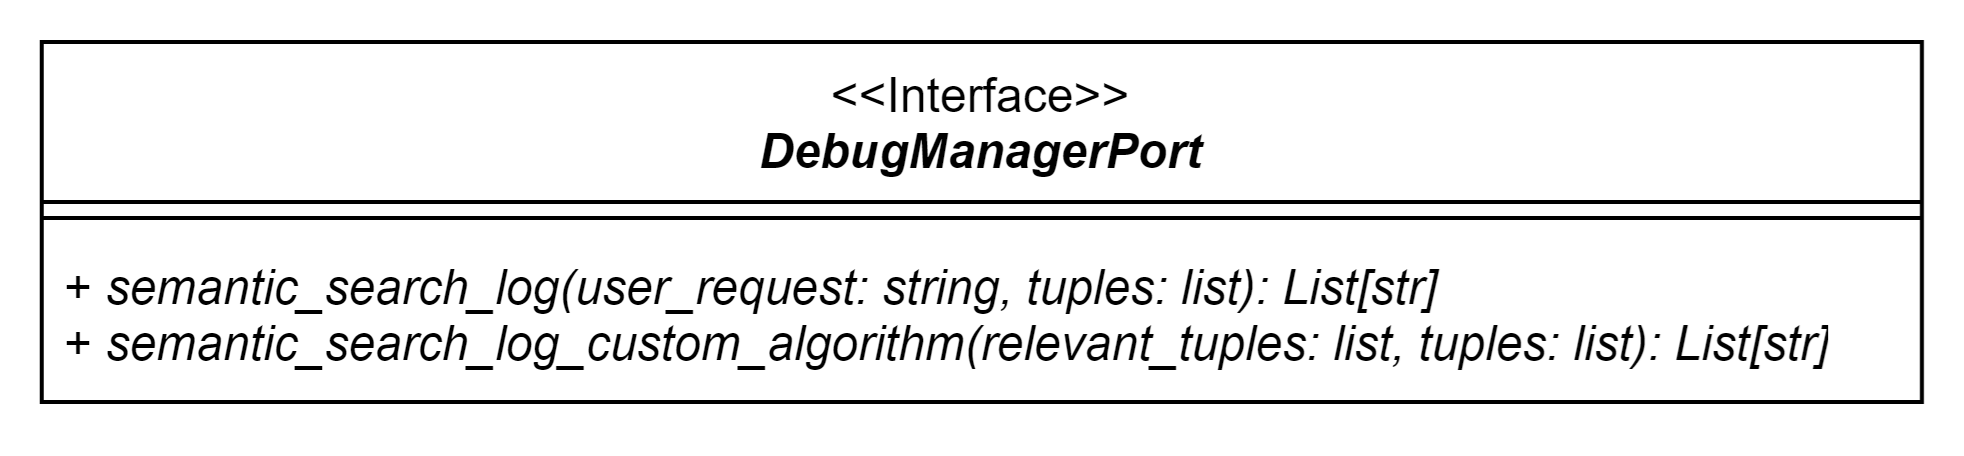
\includegraphics[width=0.6\textwidth]{assets/Backend/debug_manager_port.png}
    \caption{Diagramma dell'interfaccia DebugManagerPort}
  \end{figure}
\begin{itemize}
    \item \textbf{Descrizione}: DebugManagerPort definisce il contratto per la gestione dei log relativi alle operazioni di ricerca semantica;
    \item \textbf{Operazioni}:
    \begin{itemize}
      \item Effettua il debug di un'operazione di ricerca semantica.
    \end{itemize}
    \item \textbf{Implementazione}: i dettagli dell'implementazione sono riportati nelle classi concrete.
\end{itemize}  

\subsubsubsection{DbManagerAbstractFactory} \label{DbManagerAbstractFactory}
\begin{figure}[H]
    \centering
    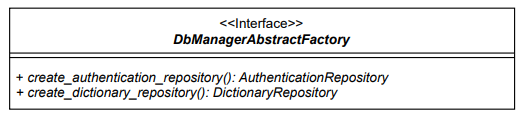
\includegraphics[width=0.6\textwidth]{assets/Backend/db_manager_abstract_factory.png}
    \caption{Diagramma dell'interfaccia DbManagerAbstractFactory}
  \end{figure}
\begin{itemize}
    \item \textbf{Descrizione}: DbManagerAbstractFactory fornisce una struttura per la creazione dei componenti relativi alla gestione dei dati dei dizionari e degli utenti;
    \item \textbf{Operazioni}:
    \begin{itemize}
      \item Creazione di un'istanza di AuthenticationRepository;
      \item Creazione di un'istanza di DictionaryRepository.
    \end{itemize}
    \item \textbf{Implementazione}: i dettagli dell'implementazione sono riportati nelle classi concrete;
    \item \textbf{Dipendenze}:
    \begin{itemize}
      \item AuthenticationRepository;
      \item DictionaryRepository.
    \end{itemize}
\end{itemize} 

\subsubsubsection{AuthenticationRepository} \label{AuthenticationRepository}
\begin{figure}[H]
    \centering
    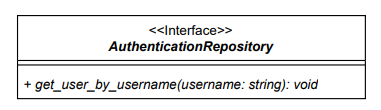
\includegraphics[width=0.6\textwidth]{assets/Backend/authentication_repository.png}
    \caption{Diagramma dell'interfaccia AuthenticationRepository}
  \end{figure}
\begin{itemize}
    \item \textbf{Descrizione}: AuthenticationRepository definisce un contratto per l'accesso e la gestione dei dati di autenticazione degli utenti;
    \item \textbf{Operazioni}: 
    \begin{itemize}
      \item Recupera i dettagli di un utente tramite lo username.
    \end{itemize}
    \item \textbf{Implementazione}: i dettagli dell'implementazione sono riportati nelle classi concrete.
\end{itemize}

\subsubsubsection{DictionaryRepository} \label{DictionaryRepository}
\begin{figure}[H]
    \centering
    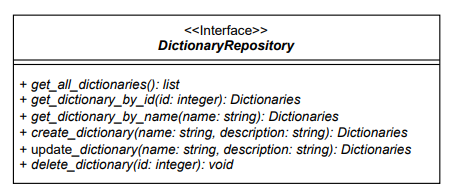
\includegraphics[width=0.6\textwidth]{assets/Backend/dictionary_repository.png}
    \caption{Diagramma dell'interfaccia DictionaryRepository}
  \end{figure}
\begin{itemize}
  \item \textbf{Descrizione}: DictionaryRepository definisce un contratto per la gestione dei dizionari all'interno del sistema; 
  \item \textbf{Operazioni}: 
    \begin{itemize}
      \item Recupero delle informazioni di tutti i dizionari;
      \item Recupero delle informazioni di un dizionario tramite il suo ID;
      \item Recupero delle informazioni di un dizionario tramite il suo nome;
      \item Creazione di un dizionario;
      \item Aggiornamento dei metadati di un dizionario;
      \item Eliminazione di un dizionario.
    \end{itemize}
  \item \textbf{Implementazione}: i dettagli dell'implementazione sono riportati nelle classi concrete.
\end{itemize} 

\subsubsubsection{FileRepository} \label{FileRepository}
\begin{figure}[H]
    \centering
    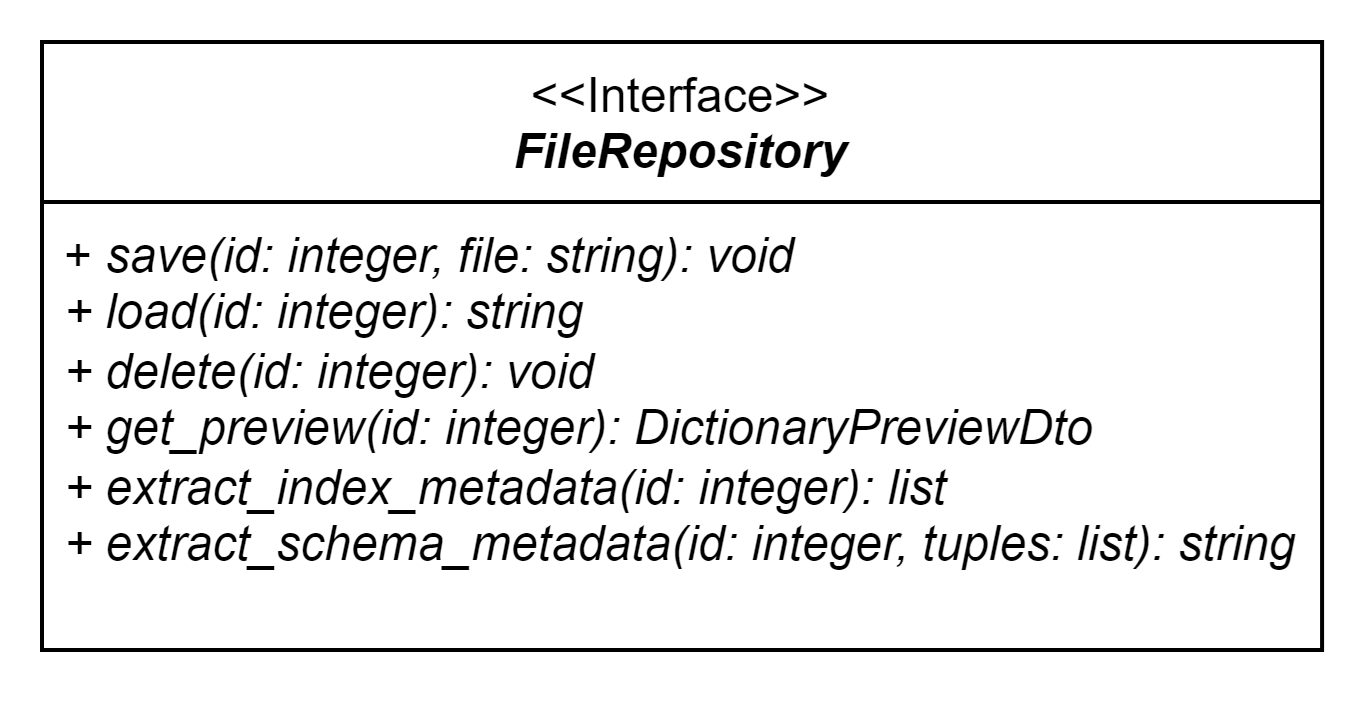
\includegraphics[width=0.6\textwidth]{assets/Backend/file_repository.png}
    \caption{Diagramma dell'interfaccia FileRepository}
  \end{figure}
\begin{itemize}
  \item \textbf{Descrizione}: questa interfaccia si occupa delle operazioni CRUD sui file dei dizionari dati.
  \item \textbf{Operazioni}: 
    \begin{itemize}
      \item Salvataggio di un file;
      \item Estrazione del contenuto di un file;
      \item Eliminazione di un file;
      \item Estrazione di un'anteprima del contenuto di un file;
      \item Estrazione dei metadati di un file per l'\glossario{indicizzazione};
      \item Estrazione dei metadati di un file in forma di \glossario{prompt}.
    \end{itemize}
  \item \textbf{Implementazione}: i dettagli dell'implementazione sono riportati nelle classi concrete.
\end{itemize} 
\subsubsection{Servizi}

\subsubsubsection{AuthenicationService} \label{AuthenticationService}
\begin{figure}[H]
    \centering
    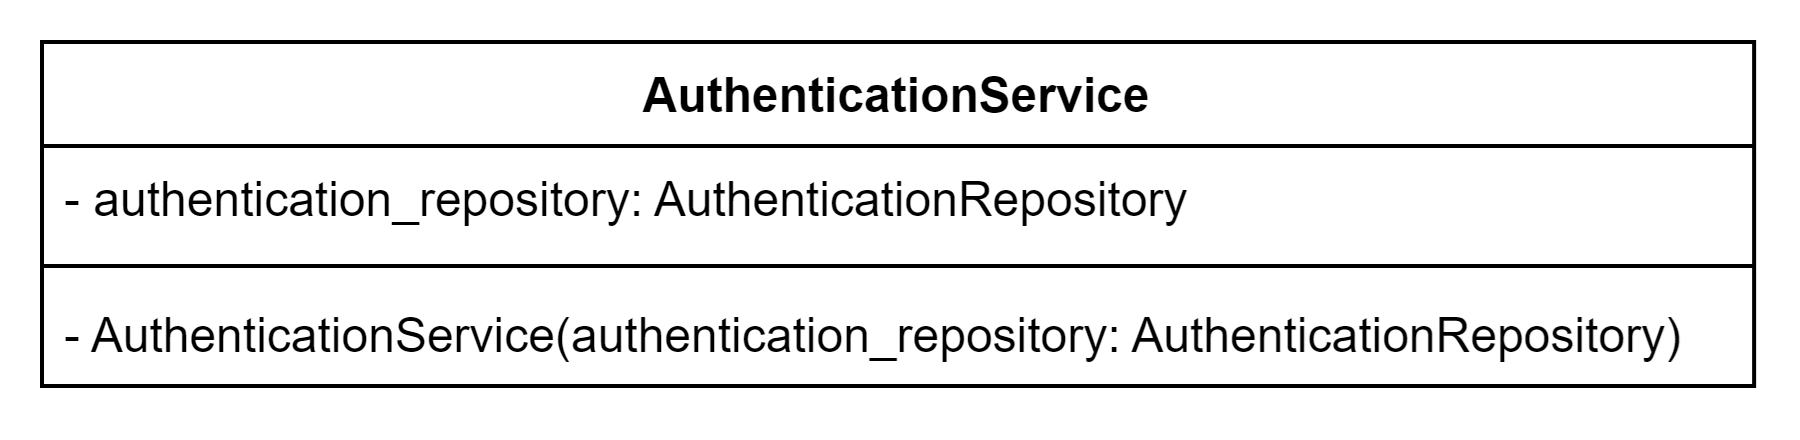
\includegraphics[width=0.7\textwidth]{assets/Backend/authentication_service.png}
    \caption{Diagramma della classe AuthenticationService}
  \end{figure}
\begin{itemize}
    \item \textbf{Descrizione}: AuthenticationService implementa il caso d'uso di autenticazione;
    \item \textbf{Interfaccia implementata}: \hyperref[AuthenticationUseCase]{AuthenticationUseCase};
    \item \textbf{Attributi}:
    \begin{itemize}
        \item \texttt{authentication\_repository}: istanza della classe utilizzata per gestire gli utenti nel sistema.
    \end{itemize}
    \item \textbf{Metodi}: 
    \begin{itemize}
        \item \texttt{AuthenicationService(authentication\_repository: AuthenticationRepository)}: costruttore della classe;
        \item \texttt{+ login(username: string, password: string)}: autentica un utente basandosi sullo username e sulla password forniti. Restituisce un oggetto di risposta che include un messaggio di stato e, in caso di successo, il token di autenticazione.
    \end{itemize}
    \item \textbf{Dipendenze}:
    \begin{itemize}
        \item AuthenticationRepository.
    \end{itemize}
\end{itemize}  

\subsubsubsection{DictionaryService} \label{DictionaryService}
\begin{figure}[H]
    \centering
    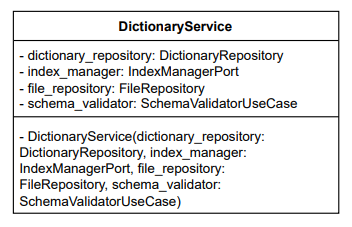
\includegraphics[width=0.8\textwidth]{assets/Backend/dictionary_service.png}
    \caption{Rappresentazione della classe DictionaryService}
  \end{figure}
\begin{itemize}
    \item \textbf{Descrizione}: DictionaryService è responsabile della gestione dei \glossario{dizionari dati};
    \item \textbf{Interfaccia implementata}: \hyperref[DictionaryUseCase]{DictionaryUseCase};
    \item \textbf{Attributi}:
    \begin{itemize}
        \item \texttt{dictionary\_repository}: istanza della classe utilizzata per gestire i dati dei dizionari;
        \item \texttt{index\_manager}: istanza del gestore degli \glossario{indici};
        \item \texttt{file\_repository}: istanza del gestore dei file;
        \item \texttt{schema\_validator}: istanza della classe utilizzata per validare lo schema dei dizionari.
    \end{itemize}
    \item \textbf{Metodi}:
    \begin{itemize}
        \item \texttt{DictionaryService(dictionary\_repository: DictionaryRepository, index\_manager: IndexManagerPort, file\_repository: FileRepository, schema\_validator: SchemaValidatorUseCase)}: costruttore della classe;
        \item \texttt{+ get\_dictionary\_list()}: recupera la lista di tutti i dizionari;
        \item \texttt{+ get\_dictionary\_by\_id(id: integer)}: recupera un dizionario tramite il suo id;
        \item \texttt{+ get\_dictionary\_file(id: integer)}: recupera il percorso del file tramite il suo id;
        \item \texttt{+ get\_dictionary\_preview(id: integer)}: recupera l'anteprima del dizionario tramite il suo id;
        \item \texttt{+ create\_dictionary(dictionary: DictionaryDto, content: string)}: crea un nuovo dizionario e salva il file associato;
        \item \texttt{+ update\_dictionary\_metadata(id: integer, dictionary: DictionaryDto)}: aggiorna i metadati di un dizionario esistente;
        \item \texttt{+ update\_dictionary\_file(id: integer, content: string)}: aggiorna il file di un dizionario esistente;
        \item \texttt{+ delete\_dictionary(id: integer)}: elimina un dizionario esistente, inclusi il file e l'indice associati;
        \item \texttt{- file\_size\_checker(content: string)}: controlla se la dimensione del file rientra nei limiti consentiti.
    \end{itemize}
    \item \textbf{Dipendenze}:
    \begin{itemize}
        \item DictionaryRepository;
        \item IndexManagerPort;
        \item FileRepository;
        \item SchemaValidatorUseCase.
    \end{itemize}
\end{itemize}

\subsubsubsection{PromptManagerService} \label{PromptManagementService}
\begin{figure}[H]
    \centering
    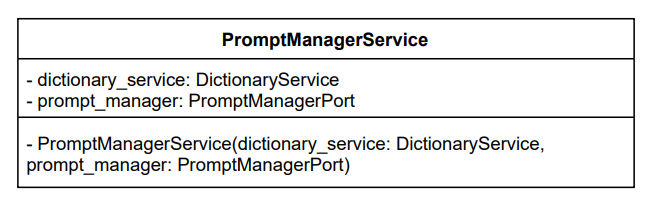
\includegraphics[width=0.8\textwidth]{assets/Backend/prompt_manager_service.png}
    \caption{Rappresentazione della classe PromptManagerService}
  \end{figure}
\begin{itemize}
    \item \textbf{Descrizione}: PromptManagerService si occupa di gestire le operazioni relative alla generazione di \glossario{prompt};
    \item \textbf{Interfaccia implementata}: \hyperref[PromptUseCase]{PromptUseCase};
    \item \textbf{Attributi}:
    \begin{itemize}
        \item \texttt{dictionary\_service}: istanza del servizio di gestione dei dizionari;
        \item \texttt{prompt\_manager}: istanza del gestore dei prompt.
    \end{itemize}
    \item \textbf{Metodi}:
    \begin{itemize}
        \item \texttt{PromptManagerService(dictionary\_service: DictionaryService, prompt\_manager: PromptManagerPort)}: costruttore della classe;
        \item \texttt{+ generate\_prompt(dictionary\_id: integer, query: string, dbms: string,\\ language: string)}: genera un prompt a partire da una richiesta, un dizionario, una lingua e un \glossario{DBMS};
        \item \texttt{+ generate\_prompt\_with\_debug(dictionary\_id: integer, query: string, \\ dbms: string, language: string)}: genera un prompt con informazioni di \glossario{debug} relative ad esso;
        \item \texttt{- generate\_prompt(dictionary\_id: integer, query: string, dbms: string,\\ language: string, log: bool)}: metodo interno per attivare la generazione del prompt utilizzando il prompt manager.
    \end{itemize}
    \item \textbf{Dipendenze}:
    \begin{itemize}
        \item DictionaryService;
        \item PromptManagerPort.
    \end{itemize}
\end{itemize}  
\subsubsubsection{Adapters - Incoming}

\paragraph{JsonSchemaValidatorAdapter} \label{JsonSchemaValidatorAdapter}
\begin{figure}[H]
    \centering
    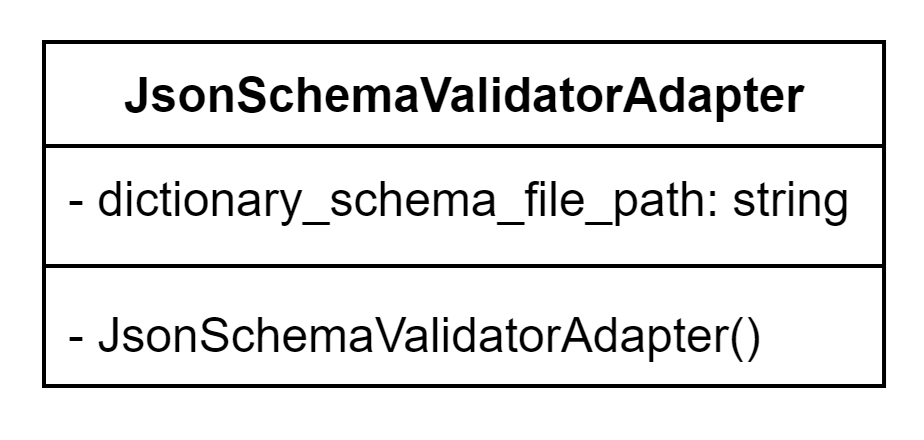
\includegraphics[width=0.95\textwidth]{assets/Backend/json_schema_validator_adapter.png}
    \caption{Rappresentazione della classe JsonSchemaValidatorAdapter}
  \end{figure}
\begin{itemize}
    \item \textbf{Descrizione:} questa classe si occupa della validazione dei \glossario{dizionari dati}.
    \item \textbf{Implementazione:} questa classe implementa l'interfaccia \hyperref[SchemaValidatorUseCase]{\texttt{SchemaValidatorUseCase}}.
    \item \textbf{Attributi:}
    \begin{itemize}
        \item \texttt{dictionary\_schema\_file\_path: string} il percorso del file contenente lo schema dei \glossario{dizionario dati}.
    \end{itemize}
    \item \textbf{Metodi:}
    \begin{itemize}
        \item \texttt{JsonSchemaValidatorAdapter(dictionary\_schema\_file\_path: string)}: costruttore della classe;
        \item \texttt{+ validate(dictionary: Dictionary): bool}: valida lo schema del dizionario passato.
    \end{itemize}
    \item \textbf{Dipendenze:}
    \begin{itemize}
        \item \texttt{Utils}
    \end{itemize}
\end{itemize} 

\paragraph{SchemaValidatorFactory} \label{SchemaValidatorFactory}
\begin{figure}[H]
    \centering
    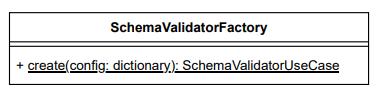
\includegraphics[width=0.95\textwidth]{assets/Backend/schema_validator_factory.png}
    \caption{Rappresentazione della classe SchemaValidatorFactory}
  \end{figure}
\begin{itemize}
    \item \textbf{Descrizione:} questa classe si occupa della creazione di istanze della classe \texttt{JsonSchemaValidatorAdapter}.
    \item \textbf{Implementazione:} questa classe non implementa alcuna interfaccia.
    \item \textbf{Attributi:} questa classe non presenta attributi.
    \item \textbf{Metodi:}
    \begin{itemize}
        \item \texttt{+ \underline{create(config: dict)}: SchemaValidatorUseCase}: crea un'istanza della classe \texttt{JsonSchemaValidatorAdapter}.
    \end{itemize}
    \item \textbf{Dipendenze:}
    \begin{itemize}
        \item \texttt{JsonSchemaValidatorAdapter}
    \end{itemize}
\end{itemize}  

\subsubsubsection{Outcoming - Adapters}

\paragraph{SqlAlchemyAuthenticationRepositoryAdapter} \label{SqlAlchemyAuthenticationRepositoryAdapter}
\begin{figure}[H]
    \centering
    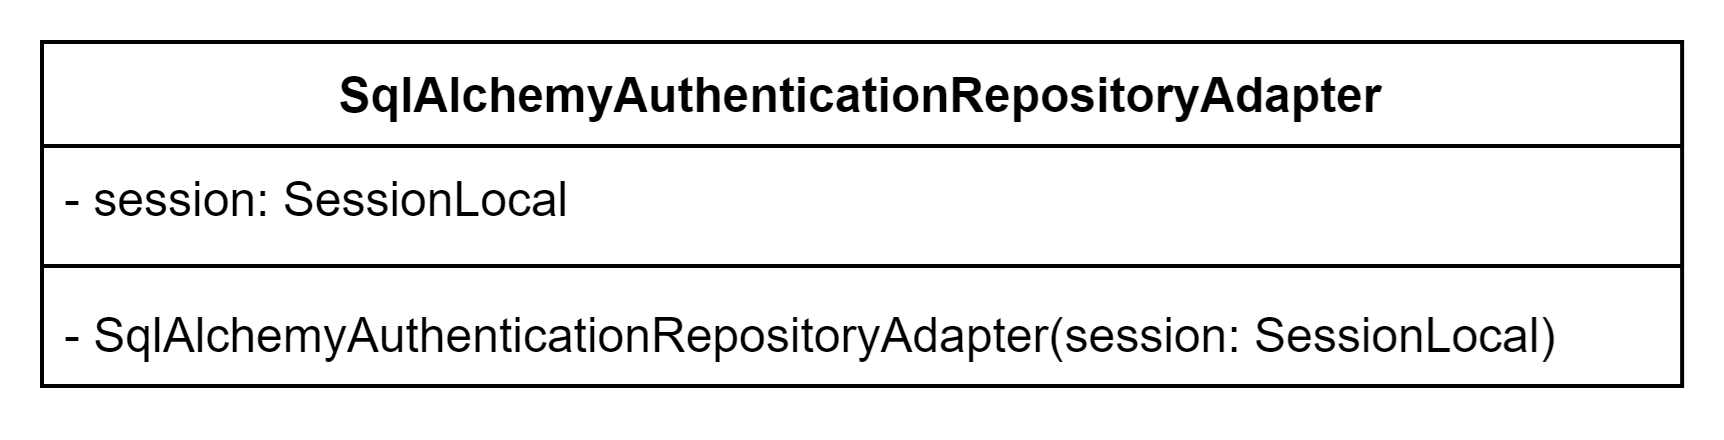
\includegraphics[width=0.95\textwidth]{assets/Backend/sql_alchemy_authentication_repository_adapter.png}
    \caption{Rappresentazione della classe SqlAlchemyAuthenticationRepositoryAdapter}
  \end{figure}
\begin{itemize}
    \item \textbf{Descrizione:} questa classe si occupa del recupero delle informazioni sugli utenti dal database.
    \item \textbf{Implementazione:} questa classe implementa l'interfaccia \hyperref[AuthenticationRepository]{\texttt{AuthenticationRepository}}.
    \item \textbf{Attributi:}
    \begin{itemize}
        \item \texttt{session: Session}: la sessione di connessione al database.
    \end{itemize}
    \item \textbf{Metodi:}
    \begin{itemize}
        \item \texttt{SqlAlchemyAuthenticationRepositoryAdapter(session: Session)}: costruttore della classe;
        \item \texttt{+ get\_user\_by\_username(username: string): AdminDto}: recupera un admin dal database tramite il suo username.
    \end{itemize}
    \item \textbf{Dipendenze:} questa classe non presenta dipendenze.
\end{itemize} 

\paragraph{SqlAlchemyDbManagerFactory} \label{SqlAlchemyDbManagerFactory}
\begin{figure}[H]
    \centering
    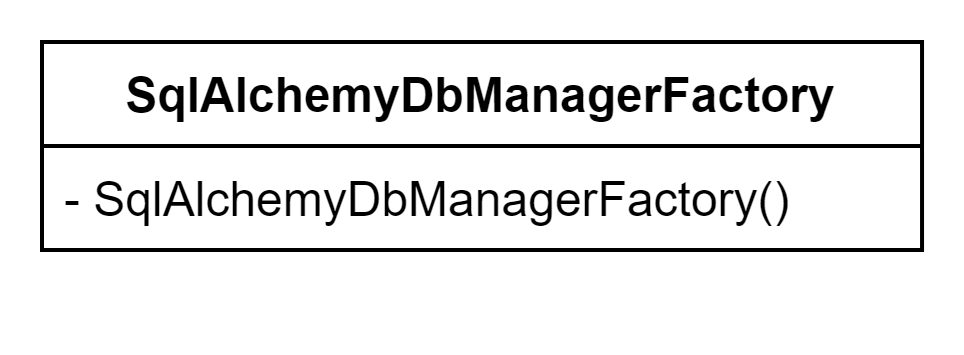
\includegraphics[width=0.95\textwidth]{assets/Backend/sql_alchemy_db_manager_factory.png}
    \caption{Rappresentazione della classe SqlAlchemyDbManagerFactory}
  \end{figure}
\begin{itemize}
    \item \textbf{Descrizione:} questa classe si occupa della costruzione delle istanze delle classi \texttt{SqlAlchemyAuthenticationRepositoryAdapter} e \texttt{SqlAlchemyDictionaryRepositoryAdapter}.
    \item \textbf{Implementazione:} questa classe implementa l'interfaccia \hyperref[DbManagerAbstractFactory]{\texttt{DbManagerAbstractFactory}}.
    \item \textbf{Attributi:} questa classe non presenta attributi.
    \item \textbf{Metodi:}
    \begin{itemize}
        \item \texttt{+ create\_authentication\_repository(): AuthenticationRepository} crea un'istanza della classe \texttt{SqlAlchemyAuthenticationRepositoryAdapter};
        \item \texttt{+ create\_dictionary\_repository(): DictionaryRepository} crea un'istanza della classe \texttt{SqlAlchemyDictionaryRepositoryAdapter}.
    \end{itemize}
    \item \textbf{Dipendenze:}
    \begin{itemize}
        \item \texttt{AuthenticationRepository};
        \item \texttt{DictionaryRepository}.
    \end{itemize}
\end{itemize}

\paragraph{SqlAlchemyDictionaryRepositoryAdapter} \label{SqlAlchemyDictionaryRepositoryAdapter}
\begin{figure}[H]
    \centering
    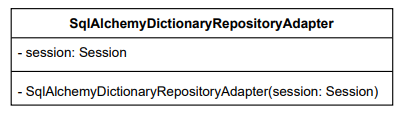
\includegraphics[width=0.95\textwidth]{assets/Backend/sql_alchemy_dictionary_repository_adapter.png}
    \caption{Rappresentazione della classe SqlAlchemyDictionaryRepositoryAdapter}
  \end{figure}
\begin{itemize}
    \item \textbf{Descrizione:} questa classe si occupa del recupero dei dizionari dati e delle operazioni CRUD su questi.
    \item \textbf{Implementazione:} questa classe implementa l'interfaccia \hyperref[DictionaryRepository]{\texttt{DictionaryRepository}}.
    \item \textbf{Attributi:}
    \begin{itemize}
        \item \texttt{session: Session}: la sessione di connessione al database.
    \end{itemize}
    \item \textbf{Metodi:}
    \begin{itemize}
        \item \texttt{SqlAlchemyDictionaryRepositoryAdapter(session: Session)}: costruttore della classe;
        \item \texttt{+ get\_all\_dictionaries(): List[DictionaryDto]}: recupera tutti i dizionari dati dal database;
        \item \texttt{+ get\_dictionary\_by\_id(id: integer): DictionaryDto}: recupera un dizionario dato il suo id;
        \item \texttt{+ get\_dictionary\_by\_name(name: string): DictionaryDto}: recupera un dizionario dato il suo nome;
        \item \texttt{+ create\_dictionary(name: string, description: string): DictionaryDto}: crea un nuovo dizionario nel database;
        \item \texttt{+ update\_dictionary(id: integer, name: string, description: string): DictionaryDto}: aggiorna un dizionario esistente nel database, dato il suo id;
        \item \texttt{+ delete\_dictionary(id: integer): void}: elimina un dizionario esistente nel database, dato il suo id.
    \end{itemize}
    \item \textbf{Dipendenze:} questa classe non presenta dipendenze.
\end{itemize} 

\paragraph{DbManagerFactory} \label{DbManagerFactory}
\begin{figure}[H]
    \centering
    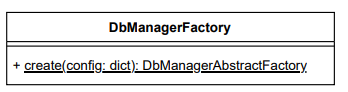
\includegraphics[width=0.95\textwidth]{assets/Backend/db_manager_factory.png}
    \caption{Rappresentazione della classe DbManagerFactory}
  \end{figure}
\begin{itemize}
    \item \textbf{Descrizione:} questa classe si occupa della creazione delle istanze della classe \texttt{DbManagerAbstractFactory} 
    \item Questa classe non implementa alcuna interfaccia.
    \item \textbf{Attributi:} questa classe non presenta attributi.
    \item \textbf{Metodi:}
    \begin{itemize}
        \item \texttt{+ create(config: dict): DbManagerAbstractFactory}: crea un'istanza della classe \texttt{DbManagerAbstractFactory}.
    \end{itemize}
    \item \textbf{Dipendenze:}
    \begin{itemize}
        \item \texttt{DbManagerAbstractFactory}
    \end{itemize}
\end{itemize}

\paragraph{TxtaiDebugManagerAdapter} \label{TxtaiDebugManagerAdapter}
\begin{figure}[H]
    \centering
    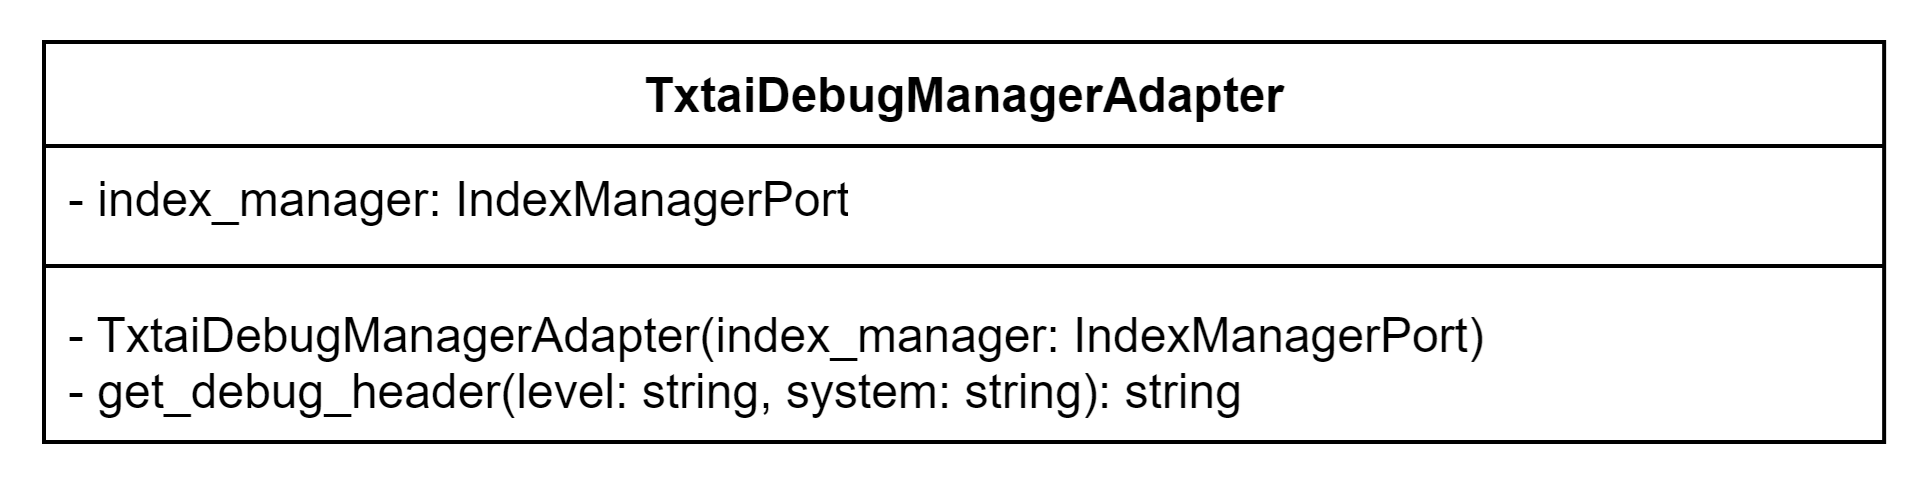
\includegraphics[width=0.95\textwidth]{assets/Backend/txtai_debug_manager_adapter.png}
    \caption{Rappresentazione della classe TxtaiDebugManagerAdapter}
  \end{figure}
\begin{itemize}
    \item \textbf{Descrizione:} questa classe si occupa della costruzione delle sezioni del documento di \glossario{log} per il \glossario{debug}.
    \item \textbf{Implementazione:} questa classe implementa l'interfaccia \hyperref[DebugManagerPort]{\texttt{DebugManagerPort}}.
    \item \textbf{Attributi:}
    \begin{itemize}
        \item \texttt{index\_manager: IndexManagerPort}: l'interfaccia di gestione degli indici;
    \end{itemize}
    \item \textbf{Metodi:}
    \begin{itemize}
        \item \texttt{TxtaiDebugManagerAdapter(index\_manager: IndexManagerPort)}: costruttore della classe;
        \item \texttt{+ semantic\_search\_log(user\_request: string, tuples: list): list} costruisce il primo pezzo documento di log, contenente le tabelle considerate nella ricerca semantica;
        \item \texttt{+ semantic\_search\_log\_custom\_algorithm(relevant\_tuples: list, tuples: list): list} costruisce il secondo pezzo del log, contenente la lista delle tabelle rilevanti;
        \item \texttt{- get\_debug\_header(): string} costruisce l'intestazione del documento di log.
    \end{itemize}
    \item \textbf{Dipendenze:}
    \begin{itemize}
        \item \texttt{IndexManagerPort}
    \end{itemize}
\end{itemize} 

\paragraph{TxtaiEmbeddingsManagerFactory} \label{TxtaiEmbeddingsManagerFactory}
\begin{figure}[H]
    \centering
    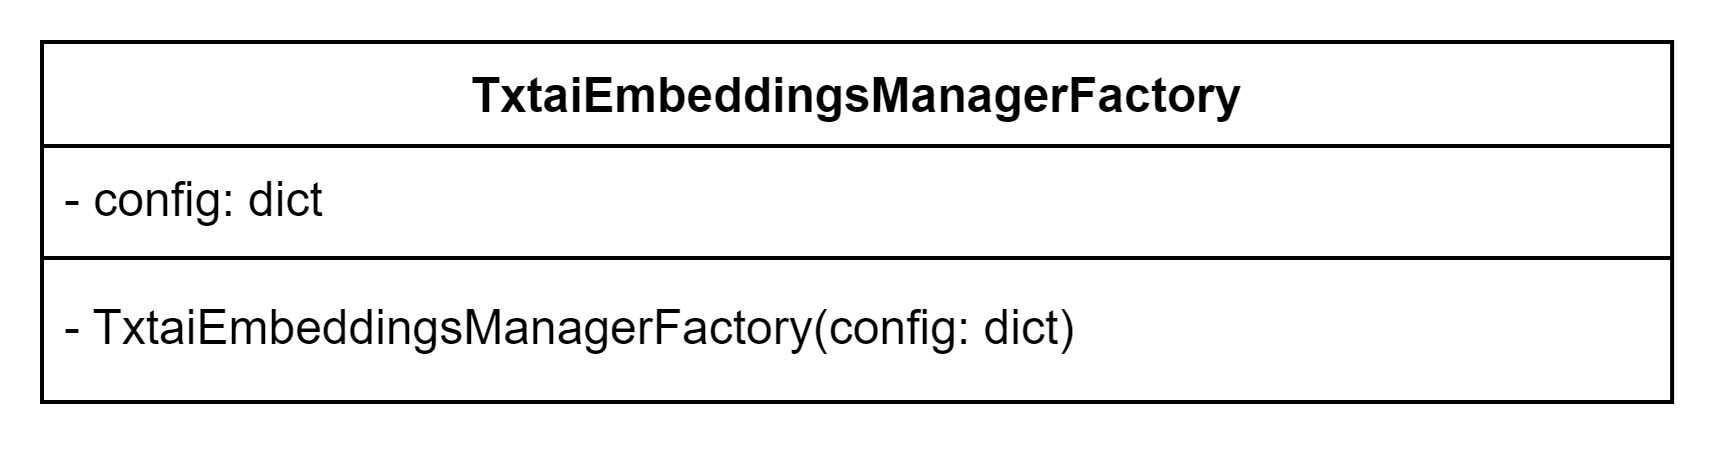
\includegraphics[width=0.95\textwidth]{assets/Backend/txtai_embeddings_manager_factory.png}
    \caption{Rappresentazione della classe TxtaiEmbeddingsManagerFactory}
  \end{figure}
\begin{itemize}
    \item \textbf{Descrizione:} questa classe si occupa della creazione dell'index manager e delle classi per la gestione dei \glossario{prompt}.
    \item \textbf{Implementazione:} questa classe implementa l'interfaccia \hyperref[EmbeddingsAbstractFactory]{\texttt{EmbeddingsAbstractFactory}}. 
    \item \textbf{Attributi:}
    \begin{itemize}
        \item \texttt{config: dict}: la configurazione del sistema;
    \end{itemize}
    \item \textbf{Metodi:}
    \begin{itemize}
        % Nella spiegazione lascio che l'istanza che viene creata è di tipo TxtaiEmbeddingsManagerFactory, ma in realtà il tipo di ritorno è l'interfaccia
        \item \texttt{TxtaiEmbeddingsManagerFactory(config: dict)}: costruttore della classe;
        \item \texttt{create\_index\_manager(file\_repository: FileRepository): IndexManagerPort}: crea un'istanza della classe \texttt{TxtaiIndexManagerAdapter};
        \item \texttt{create\_prompt\_manager\_with\_dependencies(index\_manager: IndexManagerPort, file\_repository: FileRepository): TxtaiPromptManagerAdapter}: crea un'istanza della classe \texttt{TxtaiPromptManagerAdapter} dato un indice esistente.
        \item \texttt{create\_prompt\_manager(file\_repository: FileRepository): IndexManagerPort}: crea un'istanza della classe \texttt{TxtaiPromptManagerAdapter}, creando un nuovo indice.
    \end{itemize}
    \item \textbf{Dipendenze:}
    \begin{itemize}
        % Come dipendenza la lasio verso l'interfaccia come da diagramma
        \item \texttt{FileRepository};
        \item \texttt{IndexManagerPort};
    \end{itemize}
\end{itemize} 

\paragraph{TxtaiIndexManagerAdapter} \label{TxtaiIndexManagerAdapter}
\begin{figure}[H]
    \centering
    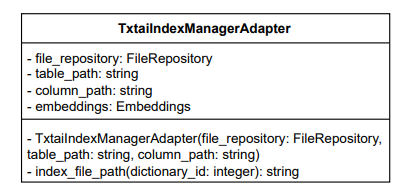
\includegraphics[width=0.95\textwidth]{assets/Backend/txtai_index_manager_adapter.png}
    \caption{Rappresentazione della classe TxtaiIndexManagerAdapter}
  \end{figure}
\begin{itemize}
    \item \textbf{Descrizione:} questa classe si occupa delle operazioni CRUD per gli indici degli embeddings.
    \item \textbf{Implementazione:} questa classe implementa l'interfaccia \hyperref[IndexManagerPort]{\texttt{IndexManagerPort}}.
    \item \textbf{Attributi:}
    \begin{itemize}
        \item \texttt{file\_repository: FileRepository}: la repository per le operazioni sui file;
        \item \texttt{table\_path: string}: il percorso al modello di generazione delle tabelle;
        \item \texttt{column\_path: string}: il percorso al modello di generazione delle colonne;
    \end{itemize}
    \item \textbf{Metodi:}
    \begin{itemize}
        \item \texttt{TxtaiIndexManagerAdapter(file\_repository: FileRepository, table\_path: string, column\_path: string)}: costruttore della classe. Si occupa anche della costruzione dell'embedding;
    \end{itemize}
    \item \textbf{Dipendenze:}
    \begin{itemize}
        \item \texttt{FileRepository}
    \end{itemize}
\end{itemize} 

\paragraph{TxtaiPromptManagerAdapter} \label{TxtaiPromptManagerAdapter}
\begin{figure}[H]
    \centering
    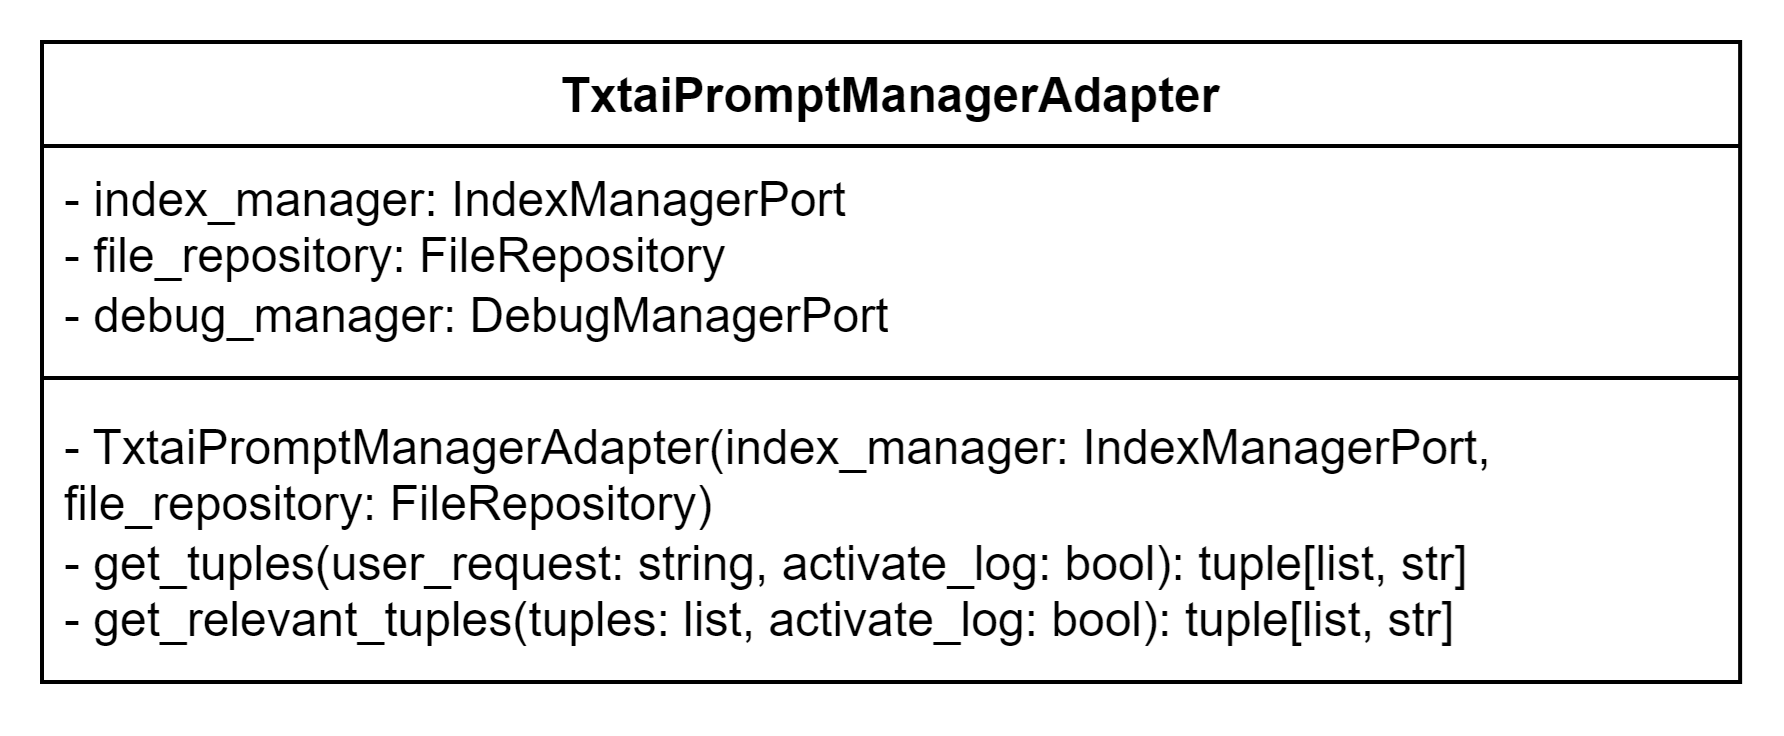
\includegraphics[width=0.95\textwidth]{assets/Backend/txtai_prompt_manager_adapter.png}
    \caption{Rappresentazione della classe TxtaiPromptManagerAdapter}
  \end{figure}
\begin{itemize}
    \item \textbf{Descrizione:} questa classe si occupa del recupero delle informazioni e la generazione del prompt.
    \item \textbf{Implementazione:} questa classe implementa l'interfaccia \hyperref[PromptManagerPort]{\texttt{PromptManagerPort}}.
    \item \textbf{Attributi:}
    \begin{itemize}
        \item \texttt{index\_manager: IndexManagerPort}: la classe di gestione degli indici;
        \item \texttt{file\_repository: FileRepository}: la repository per le operazioni sui file.
    \end{itemize}
    \item \textbf{Metodi:}
    \begin{itemize}
        \item \texttt{+ prompt\_generator(dictionary\_id: integer, user\_request: string, lang: string, dbms: string, activate\_log: bool): tuple}: crea il prompt dato l'id del dizionario dati, una richiesta in linguaggio naturale, la lingua (inglese di default) e il dbms (MariaDB di default) scelti;
        \item \texttt{+ get\_index\_manager(): IndexManagerPort}: restituisce l'istanza dell'index manager;
        \item \texttt{- create\_debug\_manager(): DebugManagerPort}: crea un'istanza del debug manager.
        \item \texttt{- get\_tuples(user\_request: string, activate\_log: bool): list}: recupera tutte le tabelle considerate nella ricerca semantica;
        \item \texttt{- get\_relevant\_tuples(tuples: list, activate\_log: bool): list}: recupera le tabelle rilevanti, cioè che superano una certa soglia di precisione, dalla ricerca semantica.
    \end{itemize}
    \item \textbf{Dipendenze:}
    \begin{itemize}
        \item \texttt{IndexManagerPort};
        \item \texttt{FileRepository};
        \item \texttt{DebugManagerPort}.
    \end{itemize}
\end{itemize} 

\paragraph{EmbeddingsManagerFactory} \label{EmbeddingsManagerFactory}
\begin{figure}[H]
    \centering
    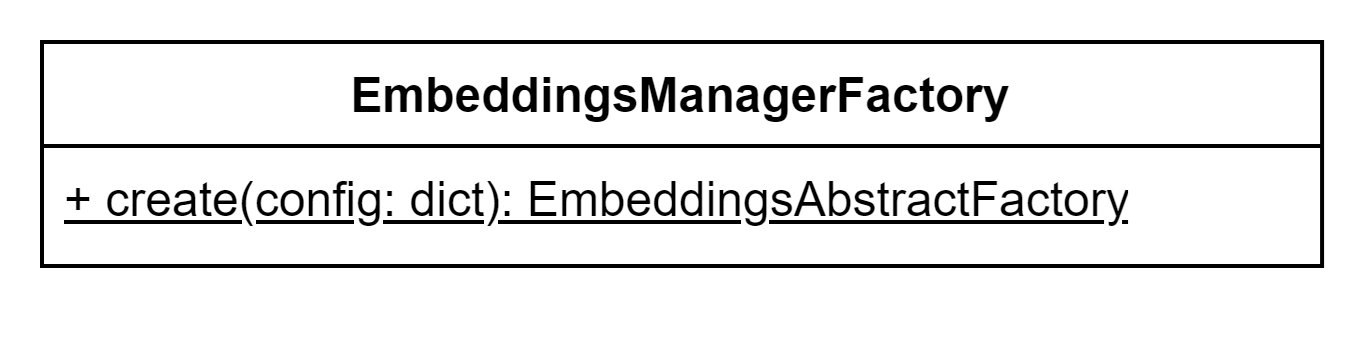
\includegraphics[width=0.95\textwidth]{assets/Backend/embeddings_manager_factory.png}
    \caption{Rappresentazione della classe EmbeddingsManagerFactory}
  \end{figure}
\begin{itemize}
    \item \textbf{Descrizione:} questa classe si occupa della costruzione di istanze della classe \texttt{EmbeddingsAbstractFactory}.
    \item \textbf{Implementazione:} questa classe non implementa alcuna interfaccia.
    \item \textbf{Attributi:} questa classe non presenta attributi.
    \item \textbf{Metodi:}
    \begin{itemize}
        \item \texttt{+ \underline{create(config: dict)}: EmbeddingsAbstractFactory}: crea un'istanza della classe \texttt{EmbeddingsAbstractFactory}.
    \end{itemize}
    \item \textbf{Dipendenze:}
    \begin{itemize}
        \item \texttt{EmbeddingsAbstractFactory}
    \end{itemize}
\end{itemize} 

\paragraph{FileFactory} \label{FileFactory}
\begin{figure}[H]
    \centering
    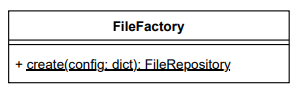
\includegraphics[width=0.95\textwidth]{assets/Backend/file_factory.png}
    \caption{Rappresentazione della classe FileFactory}
  \end{figure}
\begin{itemize}
    \item \textbf{Descrizione:} questa classe si occupa della creazione di istanze della classe \texttt{FileRepository}.
    \item \textbf{Implementazione:} questa classe non implementa alcuna interfaccia.
    \item \textbf{Attributi:} questa classe non presenta attributi.
    \item \textbf{Metodi:}
    \begin{itemize}
        \item \texttt{+ \underline{create(config: dict)}: FileRepository}: crea un'istanza della classe \texttt{FileRepository}.
    \end{itemize}
    \item \textbf{Dipendenze:}
    \begin{itemize}
        \item \texttt{FileRepository}
    \end{itemize}
\end{itemize} 

\paragraph{JsonFileAdapter} \label{JsonFileAdapter}
\begin{figure}[H]
    \centering
    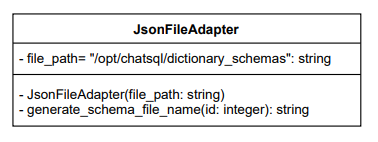
\includegraphics[width=0.95\textwidth]{assets/Backend/json_file_adapter.png}
    \caption{Rappresentazione della classe JsonFileAdapter}
  \end{figure}
\begin{itemize}
    \item \textbf{Descrizione:} questa classe si occupa delle operazioni CRUD sui file dei dizionari dati.
    \item \textbf{Implementazione:} questa classe implementa l'interfaccia \hyperref[FileRepository]{\texttt{FileRepository}}.
    \item \textbf{Attributi:}
    \begin{itemize}
        \item \texttt{file\_path: string}: il percorso al file;
    \end{itemize}
    \item \textbf{Metodi:}
    \begin{itemize}
        \item \texttt{JsonFileAdapter(file\_path: string)}: costruttore della classe;
        \item \texttt{+ save(id: integer, file: string): void}: salva il file;
        \item \texttt{+ load(id: integer): string}: carica il file del dizionario dati dall'id specificato;
        \item \texttt{+ delete(id: integer): void}: elimina il file del dizionario dati dall'id specificato;
        \item \texttt{+ get\_preview(id: integer): Union}: recupera un'anteprima del dizionario dati;
        \item \texttt{+ extract\_index\_metadata(id: integer): list}: estrae i metadati dell'indice.
        \item \texttt{+ extract\_schema\_metadata(id: integer, tuples: list): string}: seleziona le tabelle dal dizionario dati;
        \item \texttt{+ get\_json\_schema(id: integer)}: recupera le tabelle dal dizionario dati.
        \item \texttt{- generate\_schema\_file\_name(id: integer): string}: ritorna il percorso al dizionario dati. 
    \end{itemize}
    \item \textbf{Dipendenze:}
    \begin{itemize}
        \item \texttt{Utils}
    \end{itemize}
\end{itemize} 